\begin{frame}[fragile,label=matrixSquareTwoVersions]{matrix squaring}
\[ B_{ij} = \sum_{k=1}^n A_{ik}\times A_{kj} \]
\lstset{
    style=small,
    language=C,
    moredelim=**[is][\btHL<2>]{~2}{~},
    moredelim=**[is][\btHL<3>]{~3}{~},
    moredelim=**[is][\btHL<4>]{~4}{~},
}
\begin{lstlisting}
/* version 1: inner loop is k, middle is j*/
for (int i = 0; i < N; ++i)
  for (int j = 0; j < N; ++j)
    for (int k = 0; k < N; ++k)
      ~2B[i*N+j]~ += A[i * N + k] * A[k * N + j];

/* version 2: outer loop is k, middle is i */
for (int k = 0; k < N; ++k)
  for (int i = 0; i < N; ++i)
    for (int j = 0; j < N; ++j)
      B[i*N+j] += ~2A[i * N + k]~ * A[k * N + j];
\end{lstlisting}
\end{frame}

% FIXME: redraw with wider width?
\begin{frame}{performance}
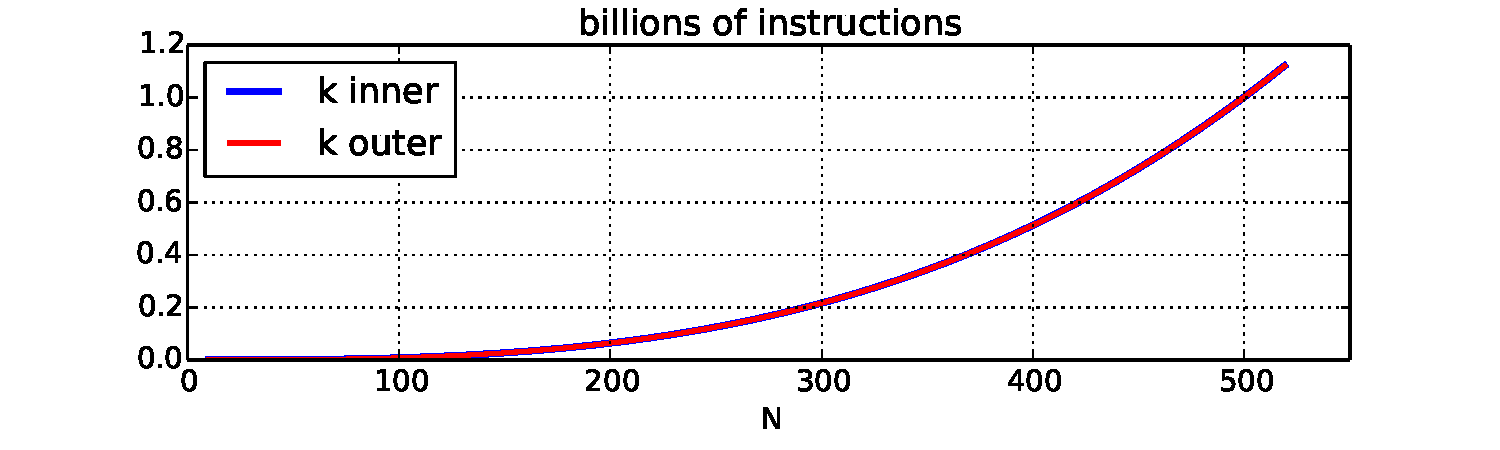
\includegraphics[width=0.99\textwidth]{../caching/k-inout-instrs} \\
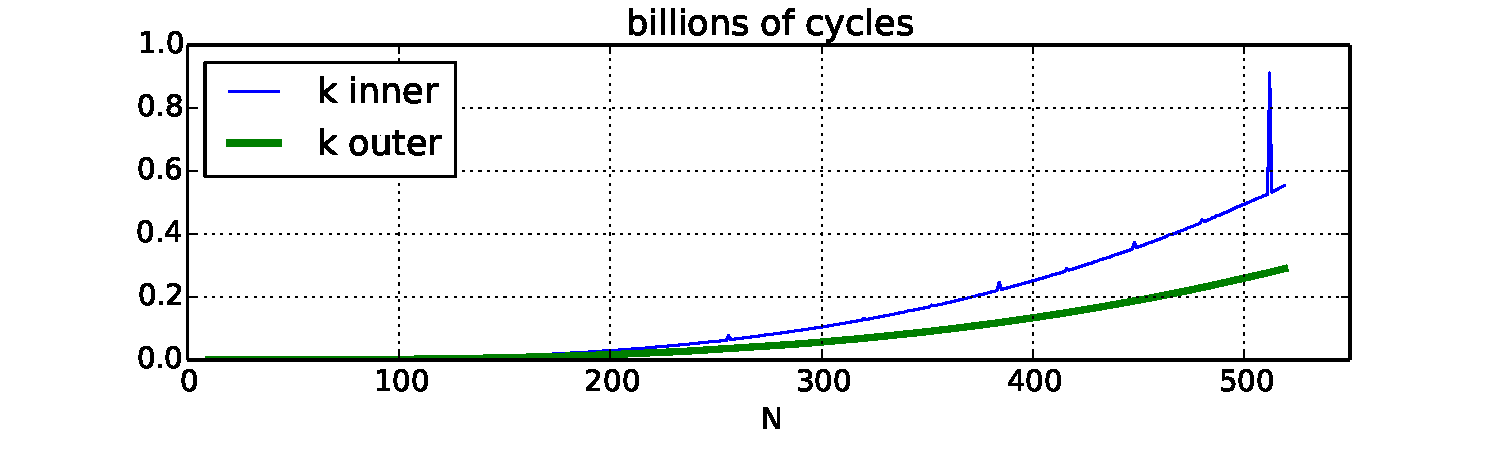
\includegraphics[width=0.99\textwidth]{../caching/k-inout-cycles}
\end{frame}

\begin{frame}{alternate view 1: cycles/instruction}
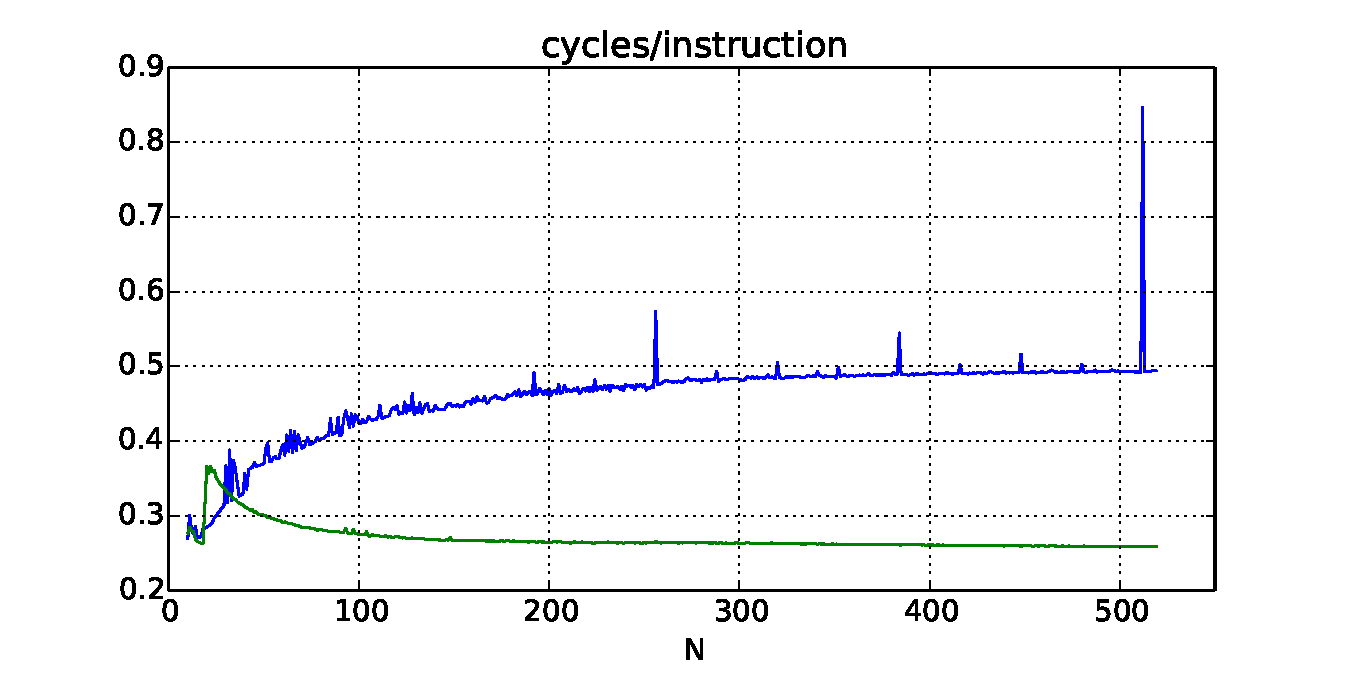
\includegraphics[width=0.99\textwidth]{../caching/k-inout-cpi}
\end{frame}

\begin{frame}{alternate view 2: cycles/operation}
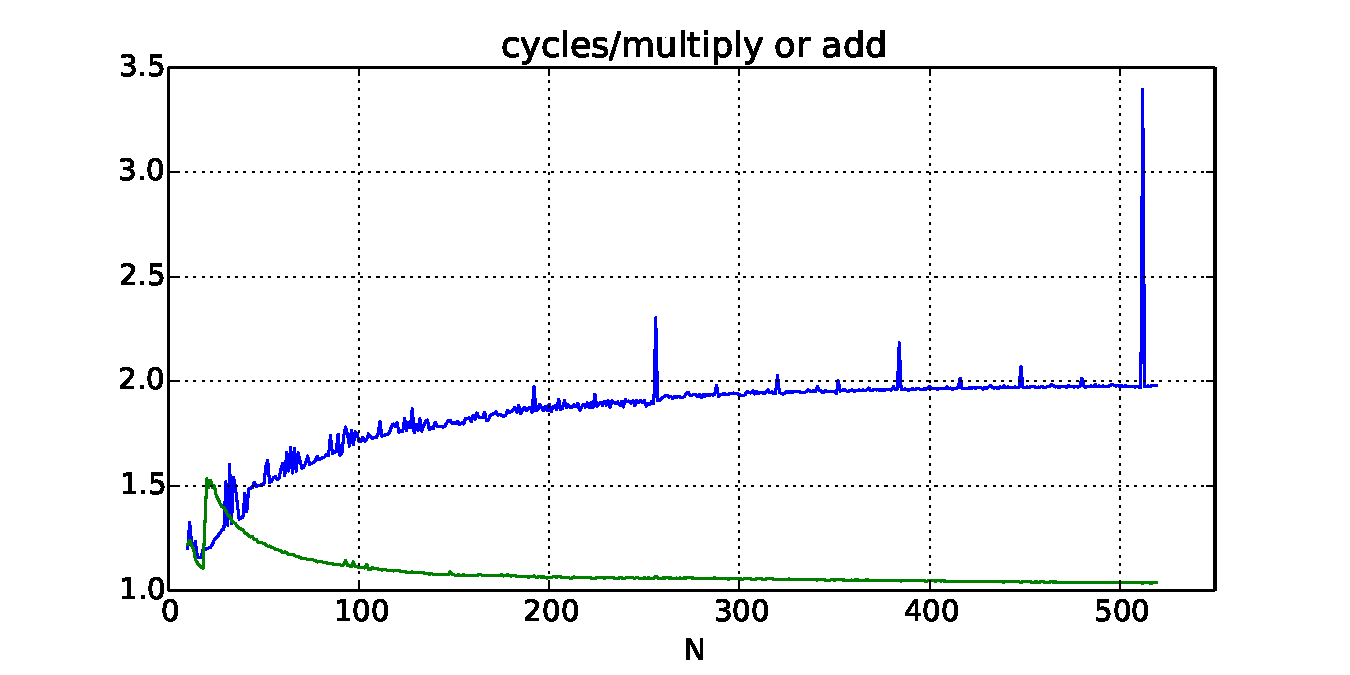
\includegraphics[width=0.99\textwidth]{../caching/k-inout-cpe}
\end{frame}

\begin{frame}{loop orders and locality}
\begin{itemize}
\item loop body: $C_{ij} += A_{ik}A_{kj}$
\item $ki\myemph<2>{j}$ order: $B_{i\myemph<2>{j}}$, $A_{k\myemph<2>{j}}$ have \myemph<1>{spatial locality}
\item $kij$ order: $A_{ik}$ has \myemph<1>{temporal locality}
\item \ldots{} better than \ldots{}
\item $ij\myemph<2>{k}$ order: $A_{i\myemph<2>{k}}$ has spatial locality
\item $ijk$ order: $B_{ij}$ has temporal locality
\end{itemize}
\end{frame}

\begin{frame}[fragile,label=matrixSquareTwoVersionsHilite]{matrix squaring}
\[ B_{ij} = \sum_{k=1}^n A_{ik}\times A_{kj} \]
\lstset{
    style=small,
    language=C,
    moredelim=**[is][\btHL<2>]{~2}{~},
    moredelim=**[is][\btHL<3>]{~3}{~},
    moredelim=**[is][\btHL<4>]{~4}{~},
}
\begin{lstlisting}
/* version 1: inner loop is k, middle is j*/
for (int i = 0; i < N; ++i)
  for (int j = 0; j < N; ++j)
    for (int k = 0; k < N; ++k)
      ~3B[i*N+j]~ += A[i * N + ~2k~] * A[k * N + j];

/* version 2: outer loop is k, middle is i */
for (int k = 0; k < N; ++k)
  for (int i = 0; i < N; ++i)
    for (int j = 0; j < N; ++j)
      B[i*N+~2j~] += ~3A[i * N + k]~ * A[k * N + ~2j~];
\end{lstlisting}
\end{frame}

\begin{frame}{L1 misses}
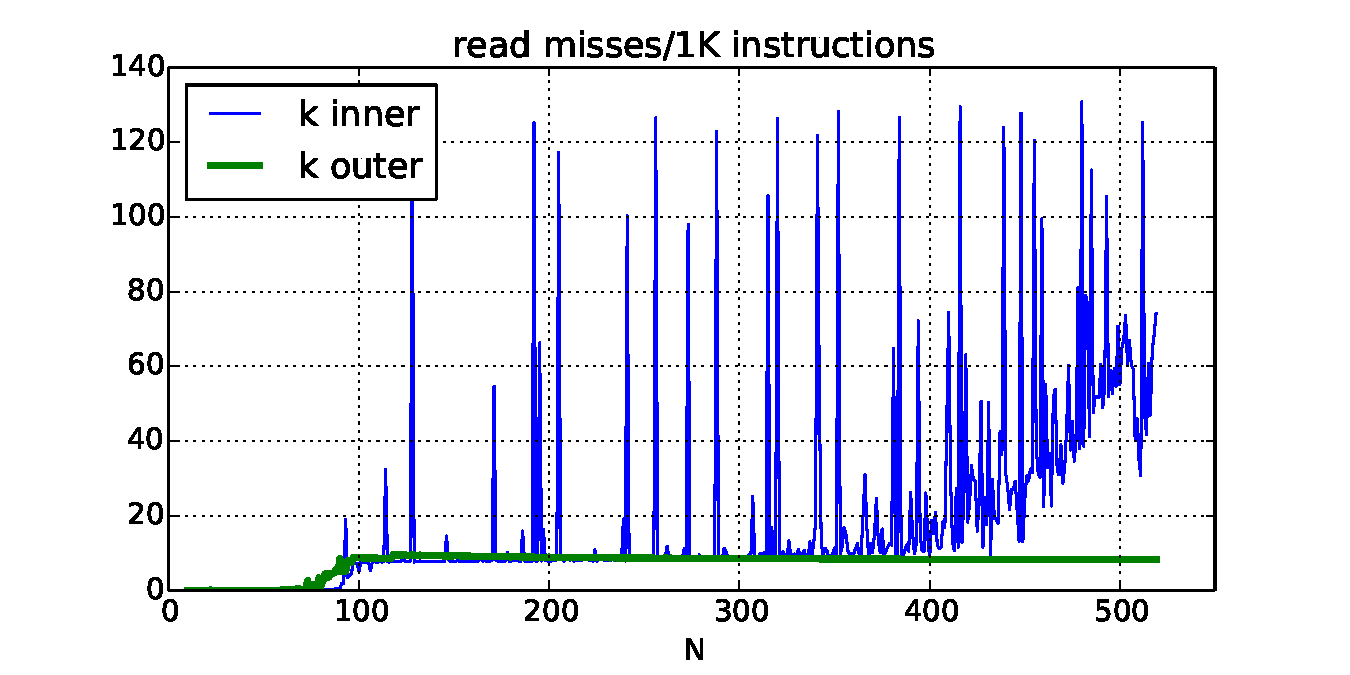
\includegraphics[width=0.99\textwidth]{../caching/k-inout-l1d_read_miss_rate}
\end{frame}

\begin{frame}{L1 miss detail (1)}
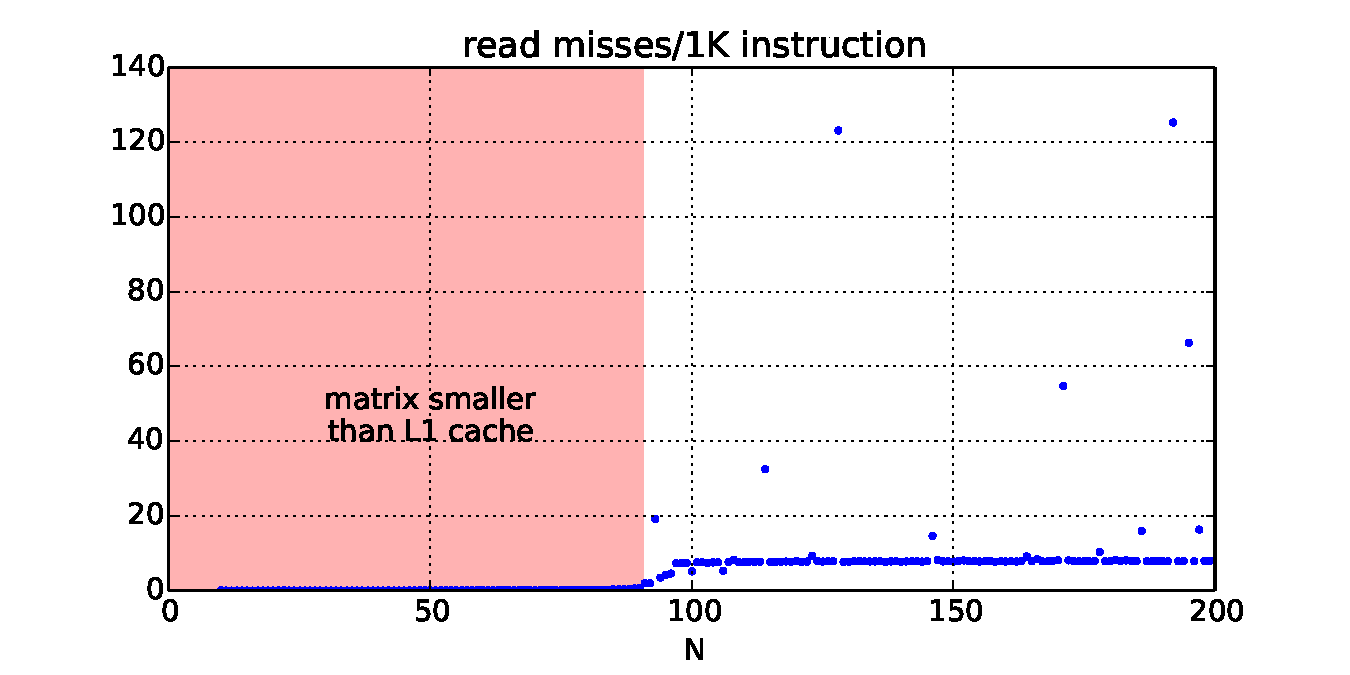
\includegraphics[width=0.99\textwidth]{../caching/k-in-l1d-miss-annot-size}
\end{frame}

\begin{frame}{L1 miss detail (2)}
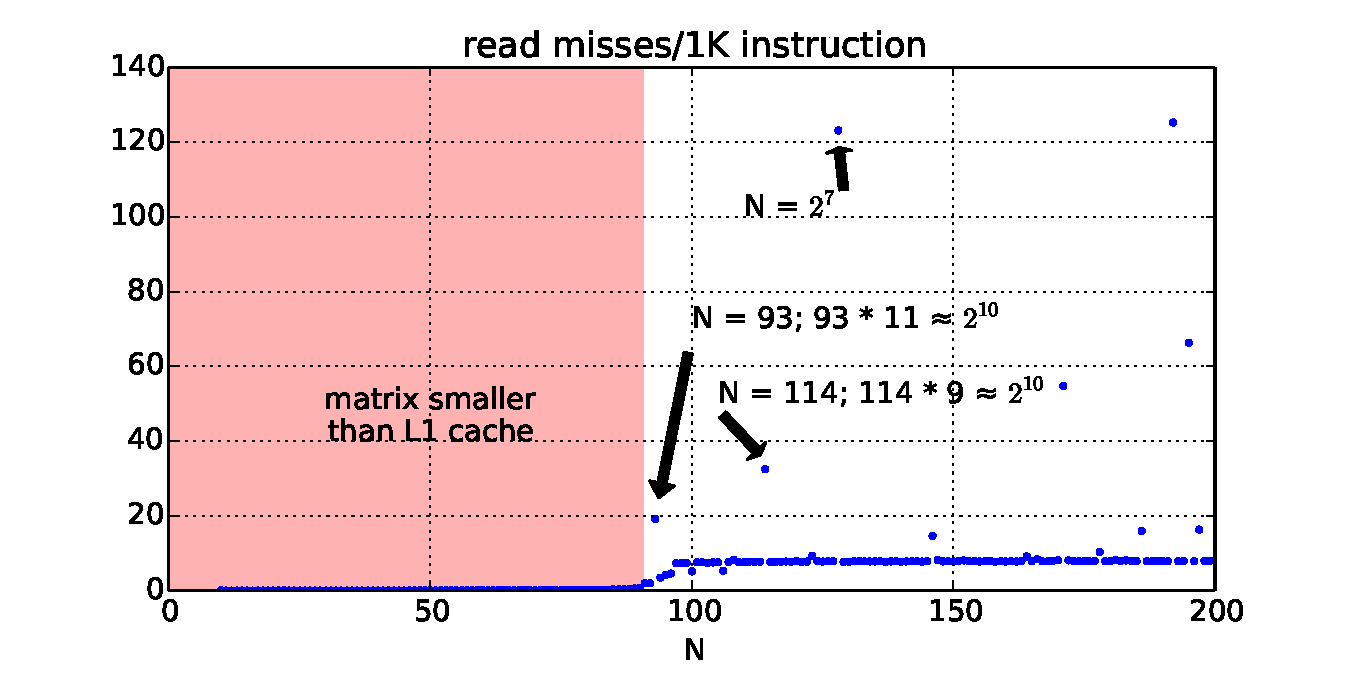
\includegraphics[width=0.99\textwidth]{../caching/k-in-l1d-miss-annot4-size}
\end{frame}

\begin{frame}[fragile,label=conflictExplainPre]{addresses}
    \begin{tabular}{lll}
        \lstinline|A[k*114+j]| &is at& \texttt{10 \textcolor<2>{blue!70!black}{\textbf<2>{0000 00}}00 0100} \\
        \lstinline|A[k*114+j+1]| &is at& \texttt{10 \textcolor<2>{blue!70!black}{\textbf<2>{0000 00}}00 1000} \\
        \lstinline|A[(k+1)*114+j]| &is at& \texttt{10 \textcolor<2>{blue!70!black}{\textbf<2>{0011 10}}01 0100} \\
        \lstinline|A[(k+2)*114+j]| &is at& \texttt{10 \textcolor<2>{blue!70!black}{\textbf<2>{0101 01}}01 1100} \\ 
        \ldots && \\
        \lstinline|A[(k+9)*114+j]| &is at& \texttt{11 \textcolor<2>{blue!70!black}{\textbf<2>{0000 00}}00 1100} \\
    \end{tabular}
    \vspace{.5cm}
    \begin{itemize}
\item<2> recall: \textcolor<2>{blue!70!black}{6 index bits}, 6 block offset bits (L1)
\end{itemize}

\end{frame}


\begin{frame}[fragile,label=conflictExplain]{conflict misses}
\begin{itemize}
\item powers of two --- lower order bits unchanged
\item \lstinline|A[k*93+j]| and \lstinline|A[(k+11)*93+j]|:
    \begin{itemize}
        \item \myemph{1023 elements apart} (4092 bytes; 63.9 cache blocks)
    \end{itemize}
\item 64 sets in L1 cache: usually maps to same set
\item \lstinline|A[k*93+(j+1)]| will not be cached (next $i$ loop)
\item even if in same block as \lstinline|A[k*93+j]|
\end{itemize}
\end{frame}
